\index{类型!族的|(}%
\index{传输|(defstyle}%
因为在类型伦中\emph{依值类型}函数是必需的, 所以也需要依值类型版的\cref{lem:map}.
然而这并不容易, 因为如果 $f:\prd{x:A} B(x)$ 和 $p:x=y$, 那么 $f(x):B(x)$ 和 $f(y):B(y)$ 是不同类型的元素, \emph{事实上}, 甚至无法询问它们是否等同.
缺失的是, $p$ 本身可以关联类型 $B(x)$ 和 $B(y)$.

已经在 \autoref{sec:identity-types} 中见过了, 它被称为 ``恒等的不可区分性''.
\index{恒等的不可区分性}%
现在为它引入不同的名字和符号, 并开始使用.

\begin{lem}[传输]
    \label{lem:transport}
    设 $P$ 是 $A$ 上的类型族, 而 $p:\id[A]xy$.
    那么有函数 $\transf{p}:P(x)\to P(y)$.
\end{lem}

\begin{proof}[第一个证明]
    令 $D:\prd{x,y:A} (\id{x}{y}) \to \type$ 为一个类型族, 其定义为
    \[D(x,y,p)\defeq P(x)\to P(y).\]
    那么有函数
    \begin{equation*}
        d\defeq\lam{x} \idfunc[P(x)]:\prd{x:A} D(x,x,\refl{x}),
    \end{equation*}
    于是对于 $p:x= y$, 归纳原理给出 $\indid{A}(D,d,x,y,p):P(x)\to P(y)$, 我们将其定义为 $\transf p$.
\end{proof}

\begin{proof}[第二个证明]
    通过归纳, 可以认为 $p$ 就是 $\refl x$.
    这个情况下, 可以令 $\transf{(\refl x)}:P(x)\to P(x)$ 为恒等函数.
\end{proof}

使用传输符号时, 有时有必要用符号表示类型族 $P$.
这种情况下, 可以写作 \[\transfib P p \blank : P(x) \to P(y).\]

回顾 $A$ 上的类型族 $P$ 可以被视作 $A$ 的元素的性质, 当 $x$ 是 $A$ 的元素而 $P(x)$ 有居留元时, 这个性质成立.
然后传输引理说 $P$ 某种意义上遵循等同, 如果 $x$ 等于 $y$, 那么当且仅当 $P(y)$ 成立时 $P(x)$ 成立.
实际上, 之后可以看到如果 $x=y$ 那么 $P(x)$ 实际上\emph{等价于} $P(y)$ .

拓扑学上, 传输引理可以被视为纤维化上的``路径提升''运算.
\index{纤维化}%
\indexdef{全!空间}%
我们认为类型族 $P:A\to \type$ 是一个\emph{纤维化}, 在底空间 $A$ 上, $P(x)$ 是 $x$ 上的纤维, $\sm{x:A}P(x)$ 是纤维化的\define{群空间}, 以及第一投影 $\sm{x:A}P(x)\to A$.
纤维化的定义的性质是给定基础空间 $A$ 的一个路径 $p:x=y$, 和经过 $x$ 的纤维上的一个点 $u:P(x)$, 可以提升路径 $p$ 到群空间, 起点为 $u$ (而这个提升的过程可以是连续的).
可以认为点 $\trans p u$ 是这个被提升的路径的另外的端点.
类型论中, 也可以定义这个路径本身:

\begin{lem}[路径提升性质]
    \label{thm:path-lifting}
    \indexdef{路径!提升}%
    \indexdef{提升!路径}%
    令 $P:A\to\type$ 为 $A$ 上的类型族, 并假设对于某些 $x:A$ 有 $u:P(x)$.
    然后对于任何 $p:x=y$, 有
    \begin{equation*}
        \mathsf{lift}(u,p):(x,u)=(y,\trans{p}{u})
    \end{equation*}
    位于 $\sm{x:A}P(x)$ 中, 于是 $\ap{\proj1}{\mathsf{lift}(u,p)} = p$.
\end{lem}
\begin{proof}
    留给读者.
    在\cref{sec:compute-sigma}会证明更通用的定理.
\end{proof}

经典同伦论中, 纤维化被定义\emph{有}路径的提升映射, ;
相比之下, 刚才展示了, 类型论中, 每个类型族都是\emph{特定的}``路径提升函数''.
这符合构造主义数学的哲学, 只有展示它, 才能说某个事物存在.
\index{类型伦中函数的连续性@类型伦中函数的``连续性''}%
它还自然地确保了路径提升被``连续地''选择, 因为类型伦中所有函数都是``连续的''.

\begin{rmk}
    尽管认为类型族 $P:A\to \type$ 是纤维化, 但一般地说``纤维化 $P:A\to\type$'' 并不是一个好主意, 为这听起来像是在说纤维化的底是 $\type$ 和群空间是 $A$.
    重复, 当一个类型族 $P:A\to \type$ 被视为一个纤维化时, 它的底是 $A$ 而群空间是 $\sm{x:A} P(x)$.

    在讨论类型族时, 偶尔会使用其它拓扑术语.
    例如, 可能会把依值函数 $f:\prd{x:A} P(x)$ 称作纤维化 $P$ 的\define{截面}
    \indexdef{截面!类型族的}%
    , 并说如果一个事物出现在所有 $P(x)$ 上, 那么说它\define{逐纤维}地发生.
    \indexdef{逐纤维}%

    例如, 截面 $f:\prd{x:A} P(x)$ 展示了 $P$ 被 ``逐纤维地居留''.
\end{rmk}

\index{函数!依值|(}
现在可以证明依值版本的\cref{lem:map}.
拓扑上的直觉是, 给定 $f:\prd{x:A} P(x)$ 和路径 $p:\id[A]xy$, 可以应用 $f$ 到 $p$ 然后得到一条路径, 它在 $P$ 的群空间上, 并 ``覆盖'' $p$ 上, 如下图所示.

\begin{center}
    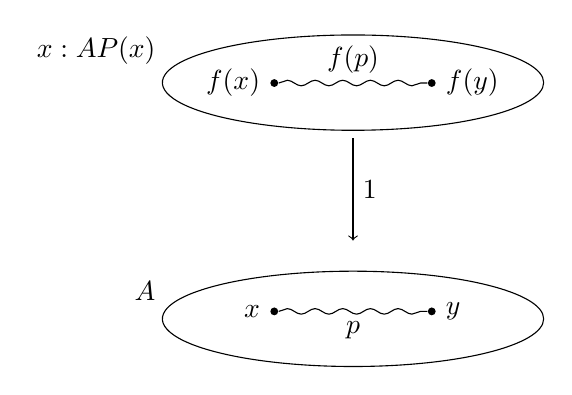
\begin{tikzpicture}[yscale=.5,xscale=2]
        \draw (0,0) arc (-90:170:8ex) node[anchor=south east] {$A$} arc (170:270:8ex);
        \draw (0,6) arc (-90:170:8ex) node[anchor=south east] {$\sm{x:A} P(x)$} arc (170:270:8ex);
        \draw[->] (0,5.8) -- node[auto] {$\proj1$} (0,3.2);
        \node[circle,fill,inner sep=1pt,label=left:{$x$}] (b1) at (-.5,1.4) {};
        \node[circle,fill,inner sep=1pt,label=right:{$y$}] (b2) at (.5,1.4) {};
        \draw[decorate,decoration={snake,amplitude=1}] (b1) -- node[auto,swap] {$p$} (b2);
        \node[circle,fill,inner sep=1pt,label=left:{$f(x)$}] (b1) at (-.5,7.2) {};
        \node[circle,fill,inner sep=1pt,label=right:{$f(y)$}] (b2) at (.5,7.2) {};
        \draw[decorate,decoration={snake,amplitude=1}] (b1) -- node[auto] {$f(p)$} (b2);
    \end{tikzpicture}
\end{center}

从 \cref{lem:map} \emph{能}得到这样的事.
给定 $f:\prd{x:A} P(x)$, 可以定义非依值函数 $f':A\to \sm{x:A} P(x)$, 通过 $f'(x)\defeq (x,f(x))$, 再考虑 $\ap{f'}{p} : f'(x) = f'(y)$.
因为 $\proj1 \circ f' \jdeq \idfunc[A]$, 根据 \cref{lem:ap-functor} 有 $\ap{\proj1}{\ap{f'}{p}} = p$; 在这个意义上 $\ap{f'}{p}$ ``覆盖'' $p$.
但是, 根据 $\ap{f'}{p}$ 的\emph{类型}, 无法明显看到, 它覆盖任意 $A$ 中的特定的路径上(本例的 $p$), 而这有时很重要.

解决方案是使用传输引理.
根据 \cref{thm:path-lifting} 有经典的路径 $\mathsf{lift}(u,p)$, 从 $(x,u)$ 到 $(y,\trans p u)$ 并覆盖 $p$.
因此, 从 $u:P(x)$ 到 $v:P(y)$ 覆盖 $p$ 的任意路径应该穿过 $\mathsf{lift}(u,p)$, 本质上唯一地, 通过从 $\trans p u$ 到 $v$ 并完全位于纤维 $P(y)$ 的路径.
因此, 上升到等价, 定义 ``从 $u$ 到 $v$ 覆盖 $p:x=y$ 的路径''  为 $P(y)$ 中的路径 $\trans p u = v$, 是有意义的.
而且, 实际上, 可以展示依值函数产生这样的路径.

\begin{lem}[依值映射]
    \label{lem:mapdep}
    \indexdef{应用!依值函数到一个路径}%
    \indexdef{路径!依值函数的应用}%
    \indexdef{函数!依值!应用到路径}%
    \indexdef{动作!路径的依值函数的}%
    提供 $f:\prd{x: A} P(x)$; 有映射
    \[\apdfunc f : \prd{p:x=y}\big(\id[P(y)]{\trans p{f(x)}}{f(y)}\big).\]
\end{lem}

\begin{proof}[第一个证明]
    令 $D:\prd{x,y:A} (\id{x}{y}) \to \type$ 为定义如下的类型族
    \begin{equation*}
        D(x,y,p)\defeq \trans p {f(x)}= f(y).
    \end{equation*}
    那么 $D(x,x,\refl{x})$ 是 $\trans{(\refl{x})}{f(x)}= f(x)$.
    而 $\trans{(\refl{x})}{f(x)}\jdeq f(x)$, 所以得到 $D(x,x,\refl{x})\jdeq (f(x)= f(x))$.
    因此, 有这个函数
    \begin{equation*}
        d\defeq\lam{x} \refl{f(x)}:\prd{x:A} D(x,x,\refl{x})
    \end{equation*}
    于是对于每个 $p:x= y$, 路径归纳可以给出 $\apdfunc f(p):\trans p{f(x)}= f(y)$ .
\end{proof}

\begin{proof}[第二个证明]
    通过归纳, 可以假定 $p$ 是 $\refl x$.
    这个情况下, 所需的等式 $\trans{(\refl{x})}{f(x)}= f(x)$ 命题地成立.
\end{proof}

在这个意义上, ``覆盖其他路径'' 的路径被笼统地称为 \emph{依值路径}.
\indexsee{依值!路径}{路径, 依值}%
\index{路径!依值}%
从 \cref{cha:hits} 开始, 它们会扮演愈发重要的角色.
\cref{sec:computational} 中, 对于一些特殊的类型族的种类, 有一些等价的方式来表示依值路径的概念, 而且有时会更方便.

现在回顾\cref{sec:pi-types}, 非依值类型函数 $f:A\to B$ 是依值函数 $f:\prd{x:A} P(x)$ 在 $P$ 是静态类型族 $P(x) \defeq B$ 的特殊情况.
这种情况下, $\apdfunc{f}$ 和 $\apfunc{f}$ 是密切相关的, 因为如下引理:

\begin{lem}
    \label{thm:trans-trivial}
    对于固定的 $B:\type$, 如果将 $P:A\to\type$ 定义为 $P(x) \defeq B$, 那么对于任何 $x,y:A$ 和 $p:x=y$ 和 $b:B$ 有路径
    \[ \transconst Bpb : \transfib P p b = b. \]
\end{lem}
\begin{proof}[第一个证明]
    固定 $b:B$, 然后令 $D:\prd{x,y:A} (\id{x}{y}) \to \type$ 为一个类型族, 定义为
    \[ D(x,y,p) \defeq (\transfib P p b = b). \]
    然后根据传输的计算规则 $D(x,x,\refl x)$ is $(\transfib P{\refl{x}}{b} = b)$ 判断等同于 $(b=b)$.
    因此, 有函数
    \[ d \defeq \lam{x} \refl{b} : \prd{x:A} D(x,x,\refl x). \]
    现在路径归纳可以给出所需的元素
    \narrowequation{
        \prd{x,y:A}{p:x=y}(\transfib P p b = b).}
\end{proof}
\begin{proof}[第二个证明]
    通过归纳, 可以假设 $y$ 是 $x$ 而且 $p$ 是 $\refl x$.
    但是 $\transfib P {\refl x} b \jdeq b$, 所以这种情况要证明的是 $b=b$, 也就是 $\refl{b}$.
\end{proof}

因此, 对于任何 $x,y:A$ 和 $p:x=y$ 和 $f:A\to B$, 通过分别连接 $\transconst Bp{f(x)}$ 和它的逆, 得到函数
\begin{align}
    \big(f(x) = f(y)\big) &\to \big(\trans{p}{f(x)} = f(y)\big)\label{eq:ap-to-apd}
    \qquad\text{和} \\
    \big(\trans{p}{f(x)} = f(y)\big) &\to \big(f(x) = f(y)\big).\label{eq:apd-to-ap}
\end{align}
事实上, 这些函数逆等价(它的意义会在\cref{sec:basics-equivalences}引入), 而且它们关联了 $\apfunc f (p)$ 和 $\apdfunc f (p)$.

\begin{lem}
    \label{thm:apd-const}
    对于 $f:A\to B$ 和 $p:\id[A]xy$, 有
    \[ \apdfunc f(p) = \transconst B p{f(x)} \ct \apfunc f (p). \]
\end{lem}
\begin{proof}[第一个证明]
    令 $D:\prd{x,y:A} (\id xy) \to \type$ 为类型族, 定义为
    \[ D(x,y,p) \defeq \big(\apdfunc f (p) = \transconst Bp{f(x)} \ct \apfunc f (p)\big). \]
    因此有
    \[D(x,x,\refl x) \jdeq \big(\apdfunc f (\refl x) = \transconst B{\refl x}{f(x)} \ct \apfunc f ({\refl x})\big).\]
    通过定义, 这个类型中出现的三个路径都是 $\refl{f(x)}$, 所以有
    \[ \refl{\refl{f(x)}} : D(x,x,\refl x). \]
    于是, 路径归纳给出所需的元素 $\prd{x,y:A}{p:x=y} D(x,y,p)$.
\end{proof}
\begin{proof}[第二个证明]
    通过归纳, 足以假定 $y$ 是 $x$ 而 $p$ 是 $\refl x$.
    这个情况下, 需要证明的是 $\refl{f(x)} = \refl{f(x)} \ct \refl{f(x)}$, 这是正确的判断.
\end{proof}

因为 $\apdfunc{f}$ 和 $\apfunc{f}$ 的类型不同, 使用不同的符号会更清晰.
% We may sometimes use a notation $\apd f p$ for $\apdfunc{f}(p)$, which is similar to the notation $\ap f p$ for $\apfunc{f}(p)$.

\index{函数!依值|)}%

至此, 希望读者开始找到一些通过恒等类型的归纳做证明的感觉.
从现在开始不再给出两种风格的证明, 而是使用更清晰和使用的 (大部分情况是更简明的第二种).
这里有一些实用的传输引理; 留给读者做证明 (用两种风格).

\begin{lem}
    \label{thm:transport-concat}
    给定 $P:A\to\type$ 和 $p:\id[A]xy$ 与 $q:\id[A]yz$ 并且 $u:P(x)$, 有
    \[ \trans{q}{\trans{p}{u}} = \trans{(p\ct q)}{u}. \]
\end{lem}

\begin{lem}
    \label{thm:transport-compose}
    对于函数 $f:A\to B$ 和类型族 $P:B\to\type$, 和任意 $p:\id[A]xy$ 与 $u:P(f(x))$, 有
    \[ \transfib{P\circ f}{p}{u} = \transfib{P}{\apfunc f(p)}{u}. \]
\end{lem}

\begin{lem}
    \label{thm:ap-transport}
    对于 $P,Q:A\to \type$ 和函数的族 $f:\prd{x:A} P(x)\to Q(x)$, 和任意 $p:\id[A]xy$ 与 $u:P(x)$, 有
    \[ \transfib{Q}{p}{f_x(u)} = f_y(\transfib{P}{p}{u}). \]
\end{lem}

\index{类型!族|)}%
\index{传输|)}